The Majumdar-Papapetrou (MP) spacetime is a static electrovacuum solution of Einstein's equations that represents a set of extremal black holes whose mutual gravitational attraction is cancelled by their mutual electromagnetic repulsion~\cite{MAJUMDAR1947,PAPAPETROU1947,HARTLE1972}.
For two black holes of masses $M_1$ and $M_2$ and electric charges $Q_1=M_1$ and $Q_2=M_2$, in equilibrium and separated by a distance $2a$ along the $z$-axis, the MP line element, in Weyl's cylindrical coordinates $(t,\rho,\phi,z)$, is given by~\cite{SMERAK2016}
\begin{equation}
  d s^2 = - \frac{d t^2}{U(\rho,z)^{2}} + U(\rho,z)^2\left[d\rho^2 + \rho^2 d\phi^2 + d z^2\right],
  \label{eq:majumdar_papapetrou_line_element}
\end{equation}
%
where
\begin{equation}
  U(\rho,z) = 1 + \frac{M_1}{\sqrt{\rho^2 + (z+a)^2}} + \frac{M_2}{\sqrt{\rho^2 + (z-a)^2}}.
  \label{eq:mp_metric_potential_cylindric}
\end{equation}
The electromagnetic potential $A_\mu$ associated with the MP solution is
\begin{equation}
  A_\mu = \left(1 - \frac{1}{U}\right) \delta_{\mu t},
  \label{eq:electromagnetic_potential_mp}
\end{equation}
where $\delta_{\mu \nu}$ is the Kronecker delta. We note that Weyl's coordinates describe only the exterior of the black holes. The event horizons and the black holes themselves are collapsed into the points $\rho=0, \, z=\pm a$. We denote the total mass of the binary system by $M_T=M_1+M_2$ and its mass ratio by $M_R=M_2/M_1$. Without loss of generality, we assume that $0 \le M_R \le 1$.

Being described by a static metric, the MP spacetime does not possess an ergosphere in the sense described in Sec.~\ref{ch:penrose_binaries:sec:penrose_review}. Consequently, the energy associated with geodesic motion in the MP spacetime is always positive, meaning that energy extraction by free particles is impossible. Charged particles, however, interact with charged black holes through Lorentz forces and, hence, do not follow geodesics.
If the electromagnetic interaction is attractive, negative energy trajectories and energy extraction are, in principle, possible. For a single charged black hole described by the RN metric, the fact that the Penrose process is viable was shown in Ref.~\cite{DENARDO1973}. Building on the notion of a generalized ergosphere~\cite{RUFFINI1971,DENARDO1973}, we shall study the motion of charged particles around the MP spacetime to investigate the possibility of negative energy motion and energy extraction.

\subsection{Motion of charged particles in MP}
\label{sec:motion}

The motion of a massive charged test particle (with charge-to-mass ratio $\mu$) in a spacetime with metric $g_{\mu \nu}$, subject to the electromagnetic potential $A_{\mu}$, is determined by the Lagrangian
\begin{equation}
  \mathcal{L} = \frac{1}{2}g_{\mu \nu}\dot{x}^\mu \dot{x}^\nu - \mu A_{\alpha}\dot{x}^\alpha,
  \label{eq:lagrangian_for_charged_particle}
\end{equation}
where $x^{\mu} = x^{\mu}(\lambda)$ denotes the position of the particle at proper time $\lambda$ and the dots represent derivatives with respect to $\lambda$. Adopting Weyl's cylindrical coordinates, and taking into account the explicit form of the MP metric, the Lagrangian above can be recast as~\cite{RYZNER2015}
%
\begin{equation}
  \mathcal{L} = \frac{1}{2}\left[-\frac{\dot{t}^2}{U^2} + U^2\left( \dot{\rho}^2 + \rho^2\dot{\phi}^2 + \dot{z}^2 \right) \right] - \mu\left(1-\frac{1}{U}\right)\dot{t}.
  \label{eq:explicit_lagrangian_for_charged_particle}
\end{equation}
%
Since the Lagrangian does not depend explicitly on $t$ and $\phi$, two constants of motion (as measured by freely-falling observers at infinity) can be readily identified. The constant associated with the time symmetry is the energy divided by the mass $m$ of the particle:
%
\begin{equation}
  E = -\del{\mathcal{L}}{\dot{t}} = \frac{\dot{t}}{U^2} + \mu\left(1-\frac{1}{U}\right).
  \label{eq:conserved_energy}
\end{equation}
%
The constant associated with the angular symmetry is the angular momentum per unit mass (with respect to the $z$ axis):
%
\begin{equation}
  L = \del{\mathcal{L}}{\dot{\phi}} = U^2 \rho^2 \dot{\phi}.
  \label{eq:conserved_momentum}
\end{equation}

Given that the particle is following a time-like trajectory, it's 4-velocity is subjected to the normalization condition
%
\begin{equation}
  \mtrtens{\mu}{\nu} \dot{x}^\mu \dot{x}^\nu = -\frac{\dot{t}^2}{U^2} + U^2\left( \dot{\rho}^2 + \rho^2\dot{\phi}^2 + \dot{z}^2 \right) = -1.
  \label{eq:4_velocity_normalization_condition_mp}
\end{equation}
%
Solving Eq.~\eqref{eq:conserved_energy} for $\dot{t}$ and Eq.~\eqref{eq:conserved_momentum} $\dot{\phi}$ and substituting the results back into Eq.~\eqref{eq:4_velocity_normalization_condition_mp}, we obtain a quadratic equation for $E$, which in turn can be solved to yield
%
\begin{equation}
  E = \mu\left(1-\frac{1}{U}\right) + \sqrt{\frac{L^2}{\rho^2U^4} + \frac{1}{U^2} + \dot{\rho}^2 + \dot{z}^2},
  \label{eq:alternative_expression_for_energy}
\end{equation}
%
where the negative root has been ignored due to the fact that $E$ must be positive for particles at infinity when $\mu = 0$ (see Ref.~\cite{RUFFINI1971} for a detailed discussion about positive and negative root states for $E$). We note that Eq.~\eqref{eq:alternative_expression_for_energy} reduces to the expression found in Ref.~\cite{DENARDO1973} for a RN black hole if the mass of one of the black holes is taken to be zero and an appropriate coordinate system, centered around the other black hole, is adopted. For convenience and later use, we rewrite Eq.~\eqref{eq:alternative_expression_for_energy} as
\begin{equation} \label{eq:effective1}
  \dot{\rho}^2 + \dot{z}^2 = E_{\mathrm {eff}}^2(\rho,z) - V_{\mathrm {eff}}(\rho,z),
\end{equation}
where
\begin{equation} \label{eq:effective2}
  E_{\mathrm {eff}}(\rho,z) = E - \mu\left(1-\frac{1}{U}\right),
\end{equation}
and
\begin{equation} \label{eq:effective3}
  V_{\mathrm {eff}}(\rho,z) =\frac{L^2}{\rho^2U^4} + \frac{1}{U^2}.
\end{equation}
Note that the quantities defined above are subject to the following constraints:
\begin{equation} \label{eq:effective_constraints}
  E_{\mathrm {eff}}(\rho,z) \ge 0, \qquad E_{\mathrm {eff}}^2(\rho,z) \ge V_{\mathrm {eff}}(\rho,z).
\end{equation}

The equations of motion are obtained directly from the Euler-Lagrange equations. After using Eqs.~\eqref{eq:conserved_energy} and \eqref{eq:conserved_momentum} to eliminate $\dot{t}$ and $\dot{\phi}$, one is left with
%
\begin{align}
  \ddot{\rho} & -\frac{L^2(U +\rho \partial_{\rho}U)}{\rho^3 U^5} + \frac{2\dot{\rho}\dot{z}\partial_{z}U - (E^2 + \dot{z}^2 - \dot{\rho}^2)\partial_{\rho}U}{U} \nonumber \\ & \hspace{1.5cm} - \frac{\mu}{U}\left(\mu-2 E+\frac{E-\mu}{U}\right)\partial_{\rho}U = 0,
  \label{eq:ode_for_rho_motion}
\end{align}
%
and
\begin{align}
  \ddot{z} - \frac{L^2\partial_{z}U}{\rho^2 U^5} & + \frac{2\dot{\rho}\dot{z}\partial_{\rho}U - (E^2 - \dot{z}^2 + \dot{\rho}^2)\partial_{z}U}{U} \nonumber \\ &-  \frac{\mu}{U}\left(\mu-2 E+\frac{ E-\mu}{U}\right)\partial_{z}U = 0,
  \label{eq:ode_for_z_motion}
\end{align}
which reduce to the equations of motion found in Ref.~\cite{ASSUMPCAO2018} for neutral particles. Together with Eqs.~\eqref{eq:conserved_energy} and \eqref{eq:conserved_momentum}, the two equations above fully determine the trajectory of a massive charged particle in the MP spacetime once appropriate initial conditions have been specified. In fact, we first specify the energy $E$, the angular momentum $L$, and the initial values for $\rho$, $z$, and $\dot z$. The initial value for $\dot{\rho}$ is determined from Eq.~\eqref{eq:alternative_expression_for_energy}. Using this information, we can solve the system of equations \eqref{eq:ode_for_rho_motion}-\eqref{eq:ode_for_z_motion} to obtain $\rho(\lambda)$ and $z(\lambda)$. The final step is the integration of Eqs.~\eqref{eq:conserved_energy} and \eqref{eq:conserved_momentum}, subject to the initial data for $t$ and $\phi$, to find $t(\lambda)$ and $\phi(\lambda)$.

\subsection{Generalized Ergosphere} \label{Sec:gen_ergo}

We want to know if charged particles can have negative energies in the MP spacetime. From Eq.~\eqref{eq:alternative_expression_for_energy} it is evident that, for fixed $\mu$, the energy is completely determined by the angular momentum $L$, and the values of $\rho$, $z$, $\dot{\rho}$ and $\dot{z}$  at any given instant of time. At a fixed position, the minimum possible energy is associated with particles at rest. Letting $\dot{\rho}=\dot{z}=0$ and $L=0$ (i.e.~$\dot{\phi}=0$), we conclude that the minimum energy (per unit mass) allowed for a particle sitting at $(t,\rho,\phi,z)$ is
\begin{equation} \label{eq:minimum_energy}
  E_{\mathrm{min}} = \mu\left(1-\frac{1}{U}\right) + \frac{1}{U}.
\end{equation}

This minimum energy will be negative if the following two conditions are satisfied: Since $U \ge 1$, $\mu$ must be negative, meaning that the charge of the particle must be opposite to the charge of the black holes. Additionally, the resting particle must be inside the spatial region determined by
\begin{equation} \label{eq:rescaled_negative_energy_condition}
  \frac{1}{\sqrt{\overline{\rho}^2 + (\overline{z}+1)^2}} + \frac{M_R}{\sqrt{\overline{\rho}^2 + (\overline{z}-1)^2}} > - \frac{1+M_R}{\overline{\mu}},
\end{equation}
where $\overline{\rho} = \rho/a$, $\overline{z} = z/a$ and $\overline \mu =  \mu M_T/a$ are dimensionless quantities. The parameter $\overline \mu$ can be understood as a measure of the potential energy (per unit particle mass) associated with the electromagnetic interaction between the particle and the binary.
The inequality above determines the generalized ergosphere of the MP spacetime: particles with opposite charge in relation to the black hole and located inside the region determined by Eq.~\eqref{eq:rescaled_negative_energy_condition} will have negative energies if their velocities are sufficiently small. Particles outside, on the other hand, will have positive energies regardless of their velocities.

\begin{figure}[h]
  \centering
  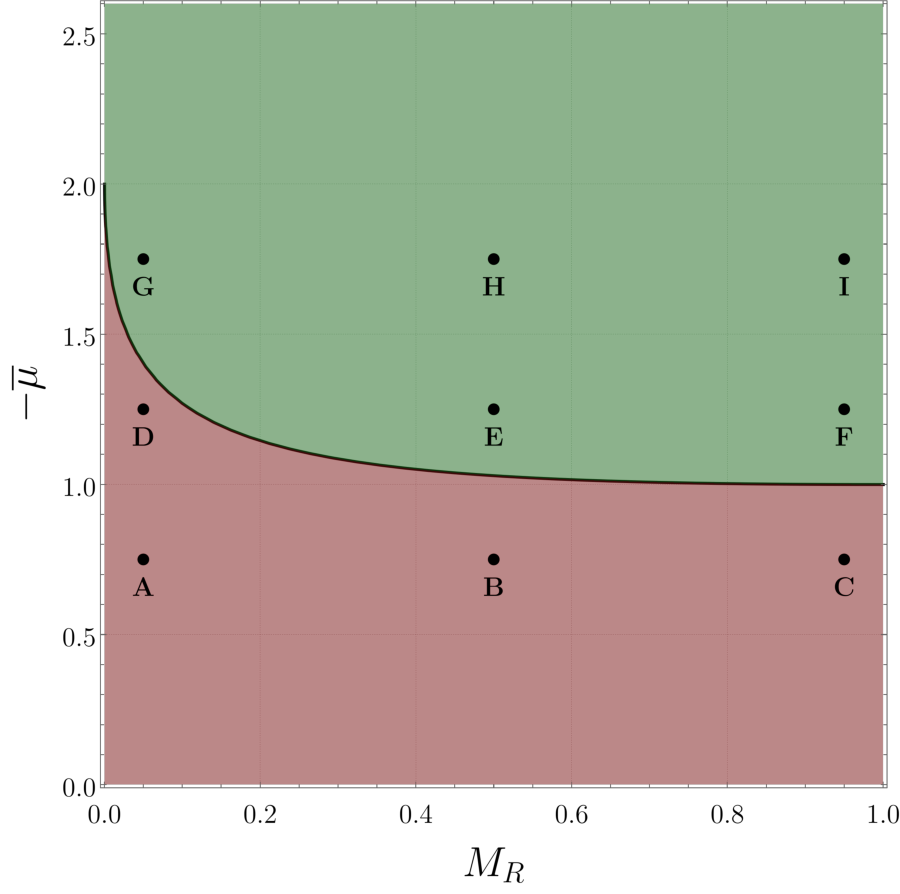
\includegraphics[scale=0.60]{img/penrose_binaries/fig1.pdf}
  \caption{The parameter space $M_R$-$\overline \mu$. The generalized ergosphere exists if and only if $\overline \mu < 0$. It consists of a single connected region for any point inside the red section. For points in the green section, on the other hand, the ergosphere is the disjoint union of two connected regions. The black curve marks the boundary between connected and disconnected ergospheres. The ergospheres associated with the black labeled dots are plotted in Fig.~\ref{fig:ergos}.}
  \label{fig:regions}
\end{figure}

Note that the notion of a generalized ergosphere depends not only on the geometry of the spacetime, but also on properties of the particle (through the charge-to-mass ratio $\mu$), as in Refs.~\cite{RUFFINI1971,DENARDO1973}. In particular, the shape of the ergosphere depends only on the parameters $M_R$ and $\overline \mu$. In order to understand this dependence, we plot the generalized ergosphere for nine $M_R$-$\overline \mu$ pairs. Each pair corresponds to a point in the parameter space of Fig.~\ref{fig:regions} and is labeled by a letter (\textbf{A}-\textbf{I}). The $\phi=0$ section of the associated ergospheres are shown in Fig.~\ref{fig:ergos}. Due to the axial symmetry of the problem, the ergospheres are the solids of revolution obtained by the rotation of the regions shown in Fig.~\ref{fig:ergos} with respect to the $\overline z$-axis. Note that the generalized ergosphere can be either a single connected region (for parameters inside the red section of Fig.~\ref{fig:regions}) or the disjoint union of two connected regions\footnote{In such a case we shall refer to each connected region as a single ergosphere.} (for parameters in the green section of Fig.~\ref{fig:regions}). The boundary separating connected and disconnected ergospheres, represented by the black line in Fig.~\ref{fig:regions}, corresponds to the saturation of Eq~\eqref{eq:rescaled_negative_energy_condition}.

\begin{figure}[h]
  \centering
  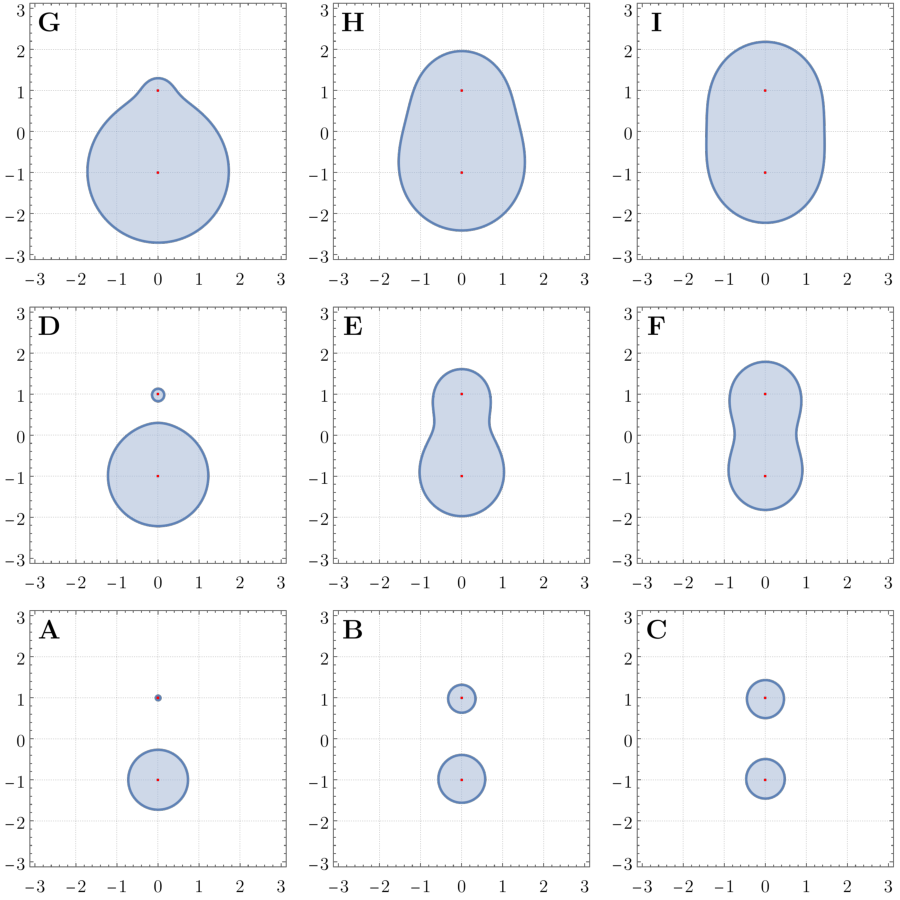
\includegraphics[scale=0.60]{img/penrose_binaries/fig2.pdf}
  \caption{The $\phi=0$ section of the ergosphere for different points (labeled \textbf{A}-\textbf{I}) in the parameter space of Fig.~\ref{fig:regions}. In each plot the horizontal and vertical axes are $\overline \rho$ and $\overline z$, respectively. The red dots indicate the location of the black holes.}
  \label{fig:ergos}
\end{figure}

The ergosphere becomes more evenly distributed around the black holes when the mass ratio $M_R$ approaches one. This is seen in Fig.~\ref{fig:regions} by following the points \textbf{A} $\rightarrow$ \textbf{B} $\rightarrow$ \textbf{C}, or \textbf{D} $\rightarrow$ \textbf{E} $\rightarrow$ \textbf{F}, or \textbf{G} $\rightarrow$ \textbf{H} $\rightarrow$ \textbf{I}. Furthermore, if $-2 < \overline \mu < -1$, we see that an increase in the mass ratio may produce a single ergosphere from two disjoint ones, as in \textbf{D} $\rightarrow$ \textbf{E}. Similarly, for any mass ratio, an increase in the absolute value of $\overline \mu$ can also induce the merger of the ergospheres, as in \textbf{D} $\rightarrow$ \textbf{G}, \textbf{B} $\rightarrow$ \textbf{E} and \textbf{C} $\rightarrow$ \textbf{F}. In fact, no matter what the mass ratio is, if $-\overline \mu$ is sufficiently small, each black hole will be surrounded by its own ergosphere. In contrast, if $-\overline \mu$ is sufficiently large, there will be a single ergosphere surrounding the binary black hole. Finally, we remark that, according to Eq.~\eqref{eq:rescaled_negative_energy_condition}, the effects of the charge of the particle, of the total mass of the binary and of the separation parameter are all combined in $\overline \mu$. Therefore, as far as the visualization of the ergosphere is concerned, the effect of increasing $|\mu|$ is exactly the same as increasing $M_T$ or decreasing $a$.

\begin{figure}[h]
  \centering
  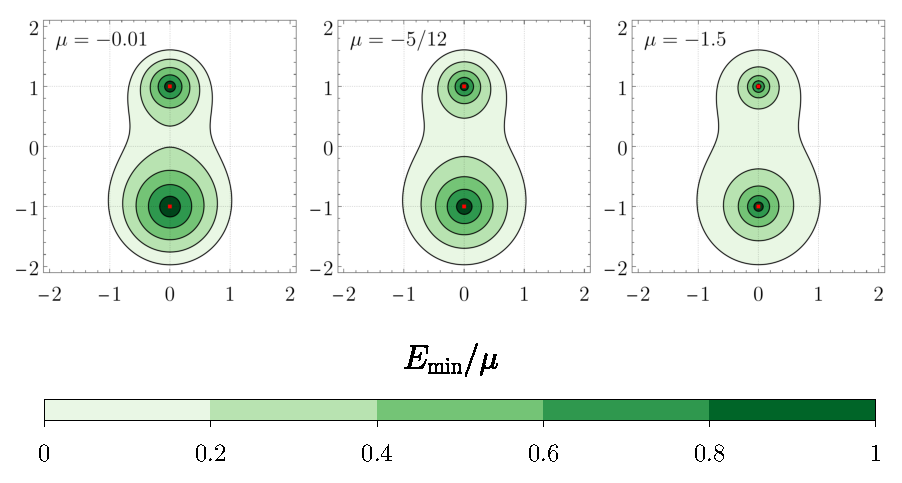
\includegraphics[scale=0.75]{img/penrose_binaries/fig3.pdf}
  \caption{Energy levels inside the generalized ergosphere of a MP black hole with $M_R=1/2$ and $\overline \mu = -5/4$, corresponding to the point \textbf{E} in Figs.~\ref{fig:regions} and \ref{fig:ergos}. The color bar represents $E_{\mathrm min}/\mu$. From left to right, the panels correspond respectively to $\mu=-0.01$, $\mu=-5/12$, and $\mu=-1.5$. The horizontal and vertical axes in each panel are $\overline \rho$ and $\overline z$, respectively. The red dots indicate the location of the black holes.}
  \label{fig:energylevels}
\end{figure}

The minimum energy (per unit mass) at a given point of the spacetime, in contrast, depends on the explicit values of $\mu$, $M_R$ and $M_T/a$. To illustrate this dependence, we plot in Fig.~\ref{fig:energylevels} the energy levels inside the ergosphere determined by $M_R=1/2$ and $\overline \mu = -5/4$ (which corresponds to the point \textbf{E} in Figs.~\ref{fig:regions} and \ref{fig:ergos}) for different combinations of $\mu$ and $M_T/a$. The color bar in Fig.~\ref{fig:energylevels} indicates the value of $E_{\mathrm{min}}/\mu$, which, according to Eq.~\eqref{eq:minimum_energy}, varies from zero (at the boundary of the ergosphere) to one (at the black holes). As $|\mu|$ decreases and $M_T/a$ increases (while $\overline \mu$ and $M_R$ are kept fixed), the shape of the ergosphere remains unchanged, but the energy levels become more evenly distributed around the black holes.

\subsection{Negative energy trajectories}
\label{sec:neg_energy}

Trajectories associated with negative energies are confined within the ergosphere defined by Eq.~\eqref{eq:rescaled_negative_energy_condition}. For a generic set of initial conditions, such paths will eventually end up at either one of the black holes. This is not much different from the case of a single RN or a Kerr black hole, in which particles with negative energies that start outside the event horizon necessarily enter the black hole and reach the spacetime singularity. Instead of focusing on this type of trajectory, we concentrated on trajectories which have no analogs in standard (Kerr and RN) black hole spacetimes~\cite{Grib:2013hxa,Zaslavskii:2020crn}. We want to investigate whether closed orbits of negative energy that live outside the black holes are allowed. It's important to first note, however, that if the Kerr black hole is immersed in an external magnetic field, closed orbits of negative energy are allowed outside the event horizon~\cite{PRASANA1982,FELICE2004}. We also note that stable circular orbits of negative energy exist around a Kerr naked singularity (and that the Penrose process can effectively take place using such orbits)~\cite{STUCHLIK1980}. We follow the procedure described in the last paragraph of section \ref{sec:motion} to solve the equations of motion. To simplify our work, we restrict our attention to two classes of planar motion and show that, by fine-tuning the initial data, one is able to find closed orbits of negative energies in the MP spacetime. These closed orbits of negative energies are unstable, in the sense that generic perturbations of the initial conditions result in trajectories that end at one of the black holes.

The first class of orbits assumes zero angular momentum ($L=0$) so that the trajectories are restricted to a plane that contains both black holes (here we choose the $\phi=0$ plane without loss of generality). For a given set of parameters $a$, $M_1$, $M_2$, $E$, and $\mu$, after fixing $\rho(0) = 0$ and $\dot{z}(0) = 0$, we fine tune the initial position $z(0)$. The initial value $\dot{\rho} (0)$ is determined from Eq.~\eqref{eq:alternative_expression_for_energy}. To illustrate, we show in Fig.~\ref{fig:orbit_closed_bh} two examples of eight-shaped orbits obtained with this scheme. The left panel of Fig.~\ref{fig:orbit_closed_bh} represents an orbit with energy (per unit mass) $E=-2/10$ and charge-to-mass ratio $\mu=-5$ for an equal mass MP binary ($M_1=M_2=1$) with separation parameter $a=1$. The trajectory starts on the $z$-axis, at $z(0) = 5.314064237978...$ (fine-tuned). One complete revolution of the trajectory, with corresponding period of $\lambda \approx 22.64$, is shown. The right panel of Fig.~\ref{fig:orbit_closed_bh}, on the other hand, exhibits an orbit of $E=-2/10$ and $\mu=-5$ for a MP binary with mass ratio $M_R=1/2$ ($M_1=2,M_2=1$) and separation parameter $a=1$. The trajectory starts on the $z$-axis, at $z(0) = 12.832155724084...$ (fine-tuned). One complete revolution of the trajectory, with corresponding period of approximately $\lambda \approx 43.28$, is shown.

\begin{figure}[h]
  \centering
  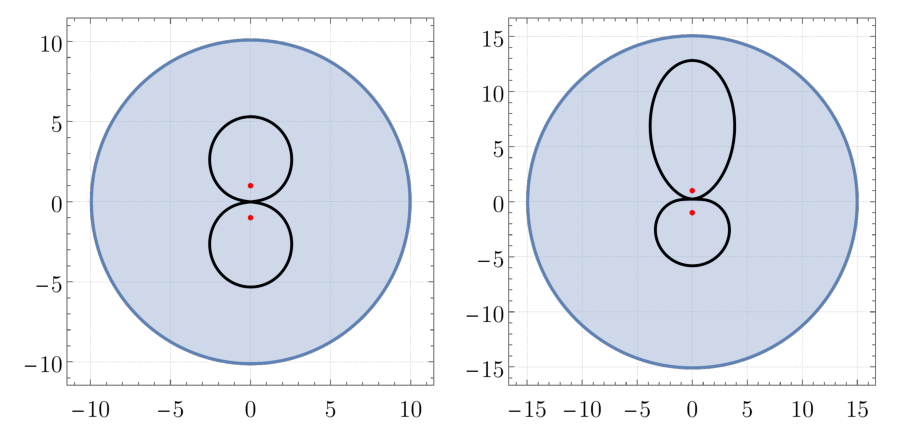
\includegraphics[scale=0.70]{img/penrose_binaries/fig4.pdf}
  \caption{Example of closed trajectories of negative energy (black curves) in the plane containing the black holes. The blue region is the generalized ergosphere of the spacetime, while the red dots indicate the location of the black holes. The horizontal and vertical axes in each panel are $\overline \rho$ and $\overline z$, respectively. Left panel: trajectory corresponding to $L=0$, $E=-2/10$, $a=M_1=M_2=1$, $\mu = -5$, $\rho(0) = 0$, $z(0) = 5.314064237978...$ (fine-tuned), and $\dot{z}(0) = 0$. The associated period of revolution is $\lambda \approx 22.64$.  Right panel: trajectory corresponding to $L=0$, $E=-2/100$, $a=1$, $M_1=2 M_2= 2$, $\mu = -5$, $\rho(0) = 0$, $z(0) = 12.832155724084...$ (fine-tuned), and $\dot{z}(0) = 0$. The associated period of revolution is $\lambda \approx 43.28$. }
  \label{fig:orbit_closed_bh}
\end{figure}

The second class of orbits is only possible for equal mass binaries and comprises trajectories that are confined to the $z=0$ plane, which is the plane equidistant to the black holes. Particles with negative energy whose motion is constrained to this plane will evolve in a perpetual oscillatory motion, either in straight lines (when $L=0$) or in more complicated precessing orbits (when $L \neq 0$). Even though these trajectories are unstable to generic perturbations, on the plane itself they are stable. In other words, infinitesimal perturbations of $\rho(0)$ and $\dot \rho(0)$ produce infinitesimal variations on the original trajectory (if $z(0)$ and $\dot z(0)$ are kept fixed).

To analyze these orbits we resort to Eqs.~\eqref{eq:effective1}-\eqref{eq:effective3}. Given $a$, $E$ and $L$, the critical points $\rho$ where $E_{\mathrm{eff}}(\rho,0)^2 = V_{\mathrm{eff}}(\rho,0)$ represent circular closed orbits. Typically, however, the particle will be confined inside a compact section of the $z=0$ plane, in a characteristic ``zoom-whirl'' orbit~\cite{ASSUMPCAO2018,Levin:2008mq}, moving between a minimum radius $\rho_{\mathrm min}$ and a maximum radius $\rho_{\mathrm max}$. In Fig.~\ref{fig:orbit_closed_z}, we show the effective energy and the effective potential for a MP spacetime with $a=1$ and $M_1 = M_2 = 1$, when the particle's charge-to-mass ratio, angular momentum (per unit mass), and energy (per unit mass) are, respectively, $\mu=-5$, $L=12.85869$, and $E=-5/100$. The particle is constrained to move between $\rho_{\mathrm min}\approx 0.543$ and $\rho_{\mathrm max}\approx 3.857$. The corresponding trajectory, assuming the starting point to be $\rho(0)=2$ and $\phi(0)=0$, is also shown in Fig.~\ref{fig:orbit_closed_z}.

\begin{figure}[h]
  \centering
  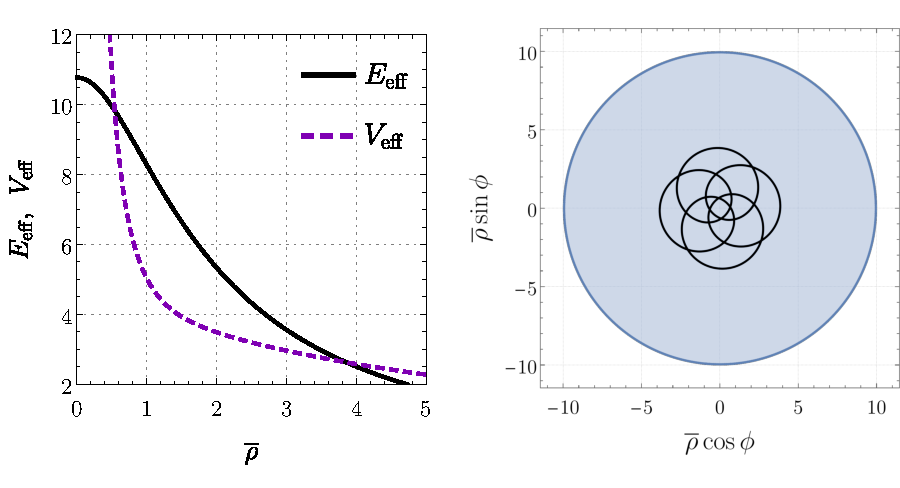
\includegraphics[scale=0.70]{img/penrose_binaries/fig5.pdf}
  \caption{Left panel: effective energy (black curve) and effective potential (purple dashed curve) for $L=12.85869$, $E=-5/100$, $a=1$, $M_1 = M_2 = 1$, $\mu = -5$. Right panel: an example of a closed trajectory of negative energy in the $z = 0$ symmetry plane. The blue region is the generalized ergosphere of the spacetime. The trajectory (black curve) is generated by setting the parameters to $L=12.85869$, $E=-5/100$, $a=1$, $M_1 = M_2 = 1$, $\mu = -5$, $\rho(0) = 2$, and $\phi(0) = 0$. The associated period of revolution is $\lambda \approx 35$.}
  \label{fig:orbit_closed_z}
\end{figure}

\subsection{Penrose Process}

Following Penrose's original proposal~\cite{PENROSE1971} and its extension to RN black holes~\cite{RUFFINI1971,DENARDO1973}, we now investigate the possibility of energy extraction from a MP binary black hole. The mechanism we shall explore is analogous to the most standard one: a negatively charged particle is sent towards the binary black hole and, once inside the generalized ergosphere, breaks up into two fragments, one of which escapes to infinity with more energy than the original particle. We assume that the incident particle follows a trajectory $T_{(0)}$, which starts outside the ergosphere and ends inside it, at the break-up point $(\rho_*,\phi_*,z_*)$. From the break-up point, two other trajectories, labeled $T_{(1)}$ and $T_{(2)}$, start. Each trajectory $T_{(i)}$ is a time-like path $x^{\mu}_{(i)}(\lambda)$ parametrized by its proper time $\lambda$. To fix notation, let $m_{(i)}$, $\mu_{(i)}$, $E_{(i)}$, $L_{(i)}$, and $P^{\mu}_{(i)}$ denote, respectively, the mass, the charge-to-mass ratio, the energy per unit mass, the angular momentum per unit mass (with respect to the z-axis), and the 4-momentum of the particle $i$ on trajectory $T_{(i)}$. We assume that fragment $1$ remains inside the ergosphere (meaning that $E_{(1)} < 0 $), while fragment $2$ escapes back to infinity.

The quantities that characterize each particle are related by conservation equations. Charge conservation, for instance, yields
\begin{equation}
  \mu_{(0)} m_{(0)}  = \mu_{(1)} m_{(1)} + \mu_{(2)} m_{(2)}.
  \label{eq:charge_conservation}
\end{equation}
The conservation of the four-momentum applied at the break-up point, on the other hand, reads
\begin{equation}
  P^{\mu}_{(0)} = P^{\mu}_{(1)} + P^{\mu}_{(2)}.
  \label{eq:four_momentum_conservation}
\end{equation}
Each component of the vector equation \eqref{eq:four_momentum_conservation} above corresponds to a different conservation equation with straightforward physical interpretation. The zero-component is just the conservation of total energy, i.e.
\begin{equation}
  E_{(0)}m_{(0)} = E_{(1)}m_{(1)} + E_{(2)}m_{(2)}.
  \label{eq:conservation_of_energy}
\end{equation}
The spatial components are the conservation of linear momenta, i.e.
\begin{equation}
  \begin{cases}
    m_{(0)}\dot{\rho}_{(0)} = m_{(1)}\dot{\rho}_{(1)} +m_{(2)}\dot{\rho}_{(2)} \\
    m_{(0)}\dot{z}_{(0)} = m_{(1)}\dot{z}_{(1)} + m_{(2)}\dot{z}_{(2)}
  \end{cases},
  \label{eq:conservation_mom_lin}
\end{equation}
and the conservation of angular momentum, i.e.
\begin{equation}
  L_{(0)}m_{(0)} = L_{(1)} m_{(1)} + L_{(2)}m_{(2)}.
  \label{eq:conservation_mom_ang}
\end{equation}
We remark that all derivatives in \eqref{eq:conservation_mom_lin} are evaluated at the break-up point. We also note that the break-up of the incident particle naturally imposes restrictions on the masses of its fragments. By squaring Eq.~\eqref{eq:four_momentum_conservation} and using the fact that the four-momentum is future-pointing and time-like, we obtain the inequality~\cite{bhat1985energetics}
\begin{equation} \label{eq:mass_constraint}
  m_{(1)}^2 + m_{(2)}^2 < m_{(0)}^2.
\end{equation}

\begin{figure}[h]
  \centering
  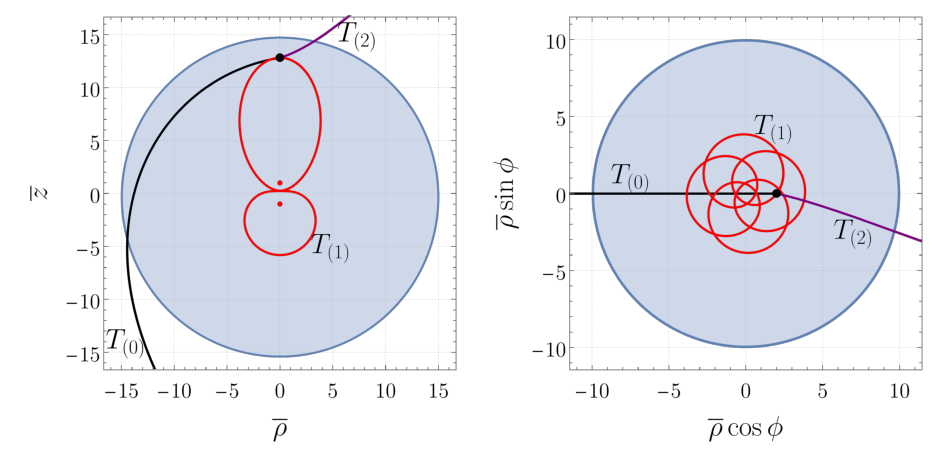
\includegraphics[scale=0.70]{img/penrose_binaries/fig6.pdf}
  \caption{Left panel: Penrose process in the $\rho$-$z$ plane of a MP spacetime with $M_1=2$, $M_2=1$, and $a=1$. Right panel: Penrose process in the $z=0$ plane of a MP spacetime with $M_1=M_2=1$ and $a=1$. In each plot, the incoming trajectory $T_{(0)}$ (black curve) splits at the black point into the negative energy orbit $T_{(1)}$ (red curve) and the trajectory of the escaping fragment $T_{(2)}$ (purple curve). The parameters that generate these trajectories are shown in Tables \ref{tab:example1} and \ref{tab:example2}. The blue region is the generalized ergosphere (for particle 1) and the red dots indicate the location of the black holes.}
  \label{fig:example1}
\end{figure}

\begin{table}[h]
  \centering
  \begin{tabular}{ccccccc}
    \hline\hline
    $i$ & $m_{(i)}$ & $\mu_{(i)}$ & $E_{(i)}$ & $L_{(i)}$ & $\dot{\rho}_{(i)}$ & $\dot{z}_{(i)}$ \\ \vspace{-0.3cm} \\
    0   & 1.00000   & -0.08345    & 1.00000   & 0         & 0.60000            & 0.09699         \\
    1   & 0.70000   & -5.00000    & -0.02000  & 0         & 0.41207            & 0.00000         \\
    2   & 0.23248   & 14.69629    & 4.36171   & 0         & 1.34012            & 0.41719         \\
    \hline\hline
  \end{tabular}
  \caption{Parameters that generate the trajectories $T_{(0)}$, $T_{(1)}$, and $T_{(2)}$ of the Penrose process shown in the left panel of Fig.~\ref{fig:example1}. The derivatives $\dot{\rho}_{(i)}$ and $\dot{z}_{(i)}$ are evaluated at the break-up point.}
  \label{tab:example1}
\end{table}

\begin{table}[h]
  \centering
  \begin{tabular}{ccccccc}
    \hline\hline
    $i$ & $m_{(i)}$ & $\mu_{(i)}$ & $E_{(i)}$ & $L_{(i)}$ & $\dot{\rho}_{(i)}$ & $\dot{z}_{(i)}$ \\ \vspace{-0.3cm} \\
    0   & 1.00000   & -0.27698    & 1.00000   & 0.00000   & 1.00000            & 0               \\
    1   & 0.10000   & -5.00000    & -0.05000  & 12.85870  & 1.36059            & 0               \\
    2   & 0.33342   & 0.66890     & 3.01423   & -3.85662  & 2.59116            & 0               \\
    \hline\hline
  \end{tabular}
  \caption{Parameters that generate the trajectories $T_{(0)}$, $T_{(1)}$, and $T_{(2)}$ of the Penrose process shown in the right panel of Fig.~\ref{fig:example1}. The derivatives $\dot{\rho}_{(i)}$ and $\dot{z}_{(i)}$ are evaluated at the break-up point.}
  \label{tab:example2}
\end{table}

From Eq.~\eqref{eq:conservation_of_energy}, the energy carried away by the escaping fragment is $E_{(2)}m_{(2)} = E_{(0)}m_{(0)} - E_{(1)}m_{(1)}$. Since we have assumed that $E_{(1)} < 0$, the escaping particle will carry away more energy than the incident particle had. If the negative energy fragment collapses to one of the black holes, it will directly decrease the energy associated with the black hole, as in Penrose's original proposal. If, on the other hand, the negative energy fragment remains in a closed orbit (such as the ones described in Sec.~\ref{sec:neg_energy}), where does the extra energy for the escaping fragment come from? Since the final state (binary black hole and bound particle fragment) is less energetic than the binary itself, we conclude that the extracted energy is associated with the binding energy of the binary. In other words, the presence of the bound particle fragment reduces the energy required to form a MP binary and the excess energy is transferred to the escaping fragment.


In Fig.~\ref{fig:example1} we exhibit examples of Penrose processes that include some of the negative energy orbits shown in Sec.~\ref{sec:neg_energy}. The left panel exhibits a Penrose process that takes place in the $\rho$-$z$ plane of a MP spacetime with $M_1=2$, $M_2=1$, and $a=1$. The incoming particle breaks-up at $\overline \rho=0$ and $\overline z = 5.314064237978...$ (fine-tuned). The right panel, on the other hand,  exhibits a Penrose process that occurs in the $z=0$ plane of a MP spacetime with $M_1=M_2=1$ and $a=1$. The incoming particle breaks-up at $\overline \rho=2$ and $\phi = 0$. The parameters that generate these examples and satisfy Eqs.~\eqref{eq:charge_conservation}-\eqref{eq:mass_constraint} are given in Tables \ref{tab:example1} and \ref{tab:example2}.


\subsection{Energy extraction efficiency}

The efficiency $\eta$ of the Penrose process can be defined as the ratio between the energy output and the energy input. Using Eq.~\eqref{eq:conservation_of_energy}, we have
%%
\begin{equation}
  \eta = \frac{E_{(2)}m_{(2)} - E_{(0)}m_{(0)}}{E_{(0)}m_{(0)}} = - \frac{E_{(1)}m_{(1)}}{E_{(0)}m_{(0)}}.
  \label{eq:penrose_efficiency_general}
\end{equation}
%
A natural question arises: what is the maximum efficiency of the Penrose process in a MP spacetime? Since $\eta$ is directly proportional to $E_{(1)}$ and inversely proportional to $E_{(0)}$, in order to maximize the efficiency of the process we need to make the absolute value of $E_{(1)}$ as large as possible and $E_{(0)}$ as small as possible. We also want the negative energy fragment to be as massive as possible in comparison to the mass of the incident particle. In other words, we want to extract as much energy as possible starting with as little energy as possible. We shall assume that the MP spacetime is fixed (meaning that $M_1$, $M_2$ and $a$ are known), the break-up point has been specified as $(\rho_*, z_*, \phi_*)$ and the charge-to-mass ratio $\mu_{(1)}$ is known. Given these hypotheses, we will determine how much energy can be extracted from a MP black hole and how the remaining parameters must be chosen in order to optimize the process.

First, the minimum energy for an incident particle coming from infinity, according to Eq.~\eqref{eq:alternative_expression_for_energy}, is $E_{(0)}=1$ and corresponds to the particle having zero kinetic energy at infinity. For that reason, we shall assume from now on that $L_{(0)}=0$ and $E_{(0)}=1$. Secondly, according to Eq.~\eqref{eq:minimum_energy} and the discussion in the first paragraph of Sec.~\ref{Sec:gen_ergo}, the energy per unit mass of particle $1$ is most negative if the particle is initially at rest. Therefore, at the break-up point we set
\begin{equation} \label{eq:traj1}
  \dot{\rho}_{(1)}=\dot{z}_{(1)}=\dot{\phi}_{(1)}=0,
\end{equation}
meaning that the associated angular momentum per unit mass and energy per unit mass are, respectively, $L_{(1)}=0$ and
\begin{equation} \label{eq:penrose_neg_energy}
  E_{(1)}=E_{(1)}^{\mathrm {min}}=\mu_{(1)}\left(1 - \frac{1}{U_*} \right) + \frac{1}{U_*},
\end{equation}
where we have defined $U_*=U(\rho_*,z_*)$ for simplicity.

Let us now study the allowed values for $m_{(1)}$. The conservation of linear momenta, Eq.~\eqref{eq:conservation_mom_lin}, yields the relation
\begin{equation} \label{eq:mass2_eq1}
  m_{(2)}^2  = m_{(0)}^2 \left( \frac{\dot \rho_{(0)} ^2 +  \dot z_{(0)} ^2 }{\dot \rho_{(2)} ^2 + \dot z_{(2)} ^2 } \right) + m_{(1)}^2 \left( \frac{\dot \rho_{(1)} ^2 + \dot z_{(1)} ^2 }{\dot \rho_{(2)} ^2 + \dot z_{(2)} ^2 } \right),
\end{equation}
where all derivatives are evaluated at the break-up point.
After replacing $\dot \rho_{(i)} ^2 + \dot z_{(i)} ^2$ using Eqs.~\eqref{eq:effective1}-\eqref{eq:effective3}, and employing the conservation equations  \eqref{eq:charge_conservation}, \eqref{eq:conservation_of_energy} and \eqref{eq:conservation_mom_ang}, the expression above reduces to
\begin{equation} \label{eq:mass2_eq2}
  m_{(2)} = \sqrt{m_{(0)}^2 - 2 m_{(0)} m_{(1)} \alpha_{(0)} + m_{(1)}^2},
\end{equation}
where
\begin{equation} \label{eq:alpha_definition}
  \alpha_{(0)} =  U_* \left[ 1 - \mu_{(0)}\left(1 - \frac{1}{U_*}\right) \right].
\end{equation}
Note that the expression between brackets in the definition of $\alpha_{(0)}$ is precisely the effective energy of the incident particle evaluated at the break-up point as given by Eq.~\eqref{eq:effective2}. The inequalities given in Eq.~\eqref{eq:effective_constraints}, together with the fact that $U_* \ge 1$, therefore imply that
\begin{equation} \label{eq:alpha_constraint}
  \alpha_{(0)} \ge 1,
\end{equation}
and
\begin{equation} \label{eq:mu0max}
  \mu_{(0)} \le 1.
\end{equation}

Eq.~\eqref{eq:mass2_eq2} and the fact that the masses are positive, together with the constraint imposed by Eq.~\eqref{eq:mass_constraint}, also imply that
\begin{equation}\label{eq:bound_of_m1_m0}
  0 < \frac{m_{(1)}}{m_{(0)}} < \alpha_{(0)} .
\end{equation}
%\le \sqrt{1 + \frac{L_0^2}{\rho_*^2 U_*^2}}
Since the radicand in Eq.~\eqref{eq:mass2_eq2} must be positive, the bound given by Eq.~\eqref{eq:bound_of_m1_m0} can be further refined to yield
\begin{equation} \label{eq:m1_max}
  0 < m_{(1)} < m_{(0)} \left( \alpha_{(0)} - \sqrt{\alpha_{(0)}^2 - 1} \right).
\end{equation}
Hence, the allowed range for $m_{(1)}$ is maximized when the inequalities \eqref{eq:alpha_constraint} and \eqref{eq:mu0max} are saturated. In fact, when $\mu_{(0)} \rightarrow 1$ one can choose $m_{(1)}\rightarrow m_{(0)}$, thus maximizing the ratio $m_{(1)}/m_{(0)}$ that appears in Eq.~\eqref{eq:penrose_efficiency_general}. Consequently, the efficiency of the Penrose process in a MP spacetime is bound from above according to
\begin{equation} \label{eq:eta_max_theory}
  \eta < \eta ^{b}  = -E_{(1)}^{\mathrm {min}}.
\end{equation}
%
We remark that the upper bound above is a function of $\mu_{(1)}$, the break-up point coordinates $\rho_*$ and $z_*$, and the MP parameters ($M_1$, $M_2$, and $a$). With the help of Eq.~\eqref{eq:penrose_neg_energy}, we now investigate in detail how these quantities affect the efficiency bound.

The dependence of $\eta^{b}$ on the charge-to-mass ratio $\mu_{(1)}$ is simple: $\eta^{b}$ increases linearly with $\mu_{(1)}$. The dependence of $\eta^{b}$ on the break-up point can be understood with the help of the energy levels shown in Fig.~\ref{fig:energylevels}: the efficiency bound increases as the break-up point approaches either one of the black holes. A more detailed analysis is shown in Fig.~\ref{fig:efficiency0}, where we plot $\eta^{b}$ as a function of $z_*$ for selected values of $\rho_*$ when $M_R=1/2$, $M_T=3$, and $\overline \mu_{(1)} = -5/4$ (corresponding to the energy levels shown in the middle panel of Fig.~\ref{fig:energylevels}). Note that when the break-up point is outside the ergosphere, the efficiency bound becomes negative, meaning that the escaping fragment will carry away less energy than the incident particle had. The Penrose process is most efficient if the break-up occurs exactly at either one of the event horizons, as indicated by the red dots in Fig.~\ref{fig:efficiency0}. When this happens, the upper bound is $-\mu_{(1)}$, which is in agreement with results obtained for the RN metric~\cite{bhat1985energetics,parthasarathy1986high}.

\begin{figure}[h]
  \centering
  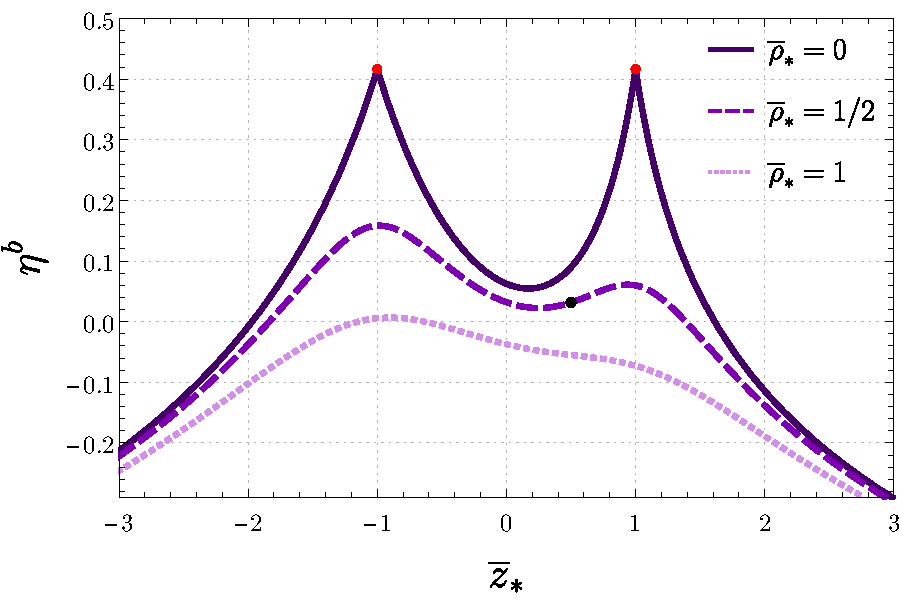
\includegraphics[scale=0.70]{img/penrose_binaries/fig7.pdf}
  \caption{Efficiency bound $\eta ^ b$ as a function of $z_*$ for $\overline \rho_*=0$ (solid curve), $\overline \rho_*=1/2$ (dashed curve), and $\overline \rho_*=1$ (dotted curve) when $M_R=1/2$, $M_T=3$, and $\overline \mu_{(1)} = -5/4$. The associated ergosphere corresponds to the point \textbf{E} in Figs.~\ref{fig:regions} and \ref{fig:ergos}, while the associated energy levels are shown in the middle panel of Fig.~\ref{fig:energylevels}. The red dots indicate the efficiency when the particle breaks-up at the black holes. The black dot shows the maximum efficiency $\eta^b = 0.03161$ for the processes represented in Fig.~\ref{fig:examplemax1} and Tables \ref{tab:max1} and \ref{tab:max2}.}
  \label{fig:efficiency0}
\end{figure}

To study the dependence of the efficiency bound on the masses of the black holes, we plot $\eta ^{b}$ as a function of the mass ratio $M_R$ when $M_T/a=3$ (top panel of Fig.~\ref{fig:efficiency2}) and as a function of $M_T/a$ when $M_R=1/2$  (top panel of Fig.~\ref{fig:efficiency3}). In both cases we have set the charge-to-mass ratio as $\mu_{(1)} = -5/12$. Each curve in these plots is associated with a different break-up point. The break-up points are shown in the bottom panels of Figs.~\ref{fig:efficiency2} and \ref{fig:efficiency3}. In the bottom panel of Fig.~\ref{fig:efficiency2}, we also exhibit the generalized ergosphere associated with a few selected values of $M_R$ (which are chosen to reproduce the ergospheres labeled \textbf{D}, \textbf{E} and \textbf{F} in Figs.~\ref{fig:regions} and \ref{fig:ergos}). Analogously, the ergospheres depicted in the bottom panel of Fig.~\ref{fig:efficiency3} (and the associated values of $M_T/a$) correspond to the ergospheres labeled \textbf{B}, \textbf{E} and \textbf{H} in Figs.~\ref{fig:regions} and \ref{fig:ergos}.

As shown in the top panel of Fig.~\ref{fig:efficiency2}, when the mass ratio $M_R$ increases (while the other parameters are kept fixed), $\eta ^{b}$ will also increase if the break-up point is closer to the lighter black hole and will decrease if the break-up point is closer to the heavier black hole. This behavior is related to the fact that the growth of $M_R$ produces an expansion of the ergosphere around the lighter companion and a reduction of the ergosphere around the heavier companion, as seen in the bottom panel of Fig.~\ref{fig:efficiency2}.
Note that the efficiency bound is independent of the mass ratio if the break-up point is equidistant to the black holes.
On the other hand, as shown in Fig.~\ref{fig:efficiency3}, when $M_T/a$ increases (while the other parameters are kept fixed), the ergosphere expands and $\eta ^{b}$ increases. We note that in the limit $M_T/a \rightarrow \infty$, no matter where the break-up occurs, the efficiency bound approaches its maximum, i.e. $\eta ^{b} \rightarrow - \mu_{(1)}$. This is explained by the fact that the distance between the break-up point and the black holes becomes negligible in comparison to the size of the ergosphere when $M_T/a \rightarrow \infty$.

\begin{figure}[h]
  \centering
  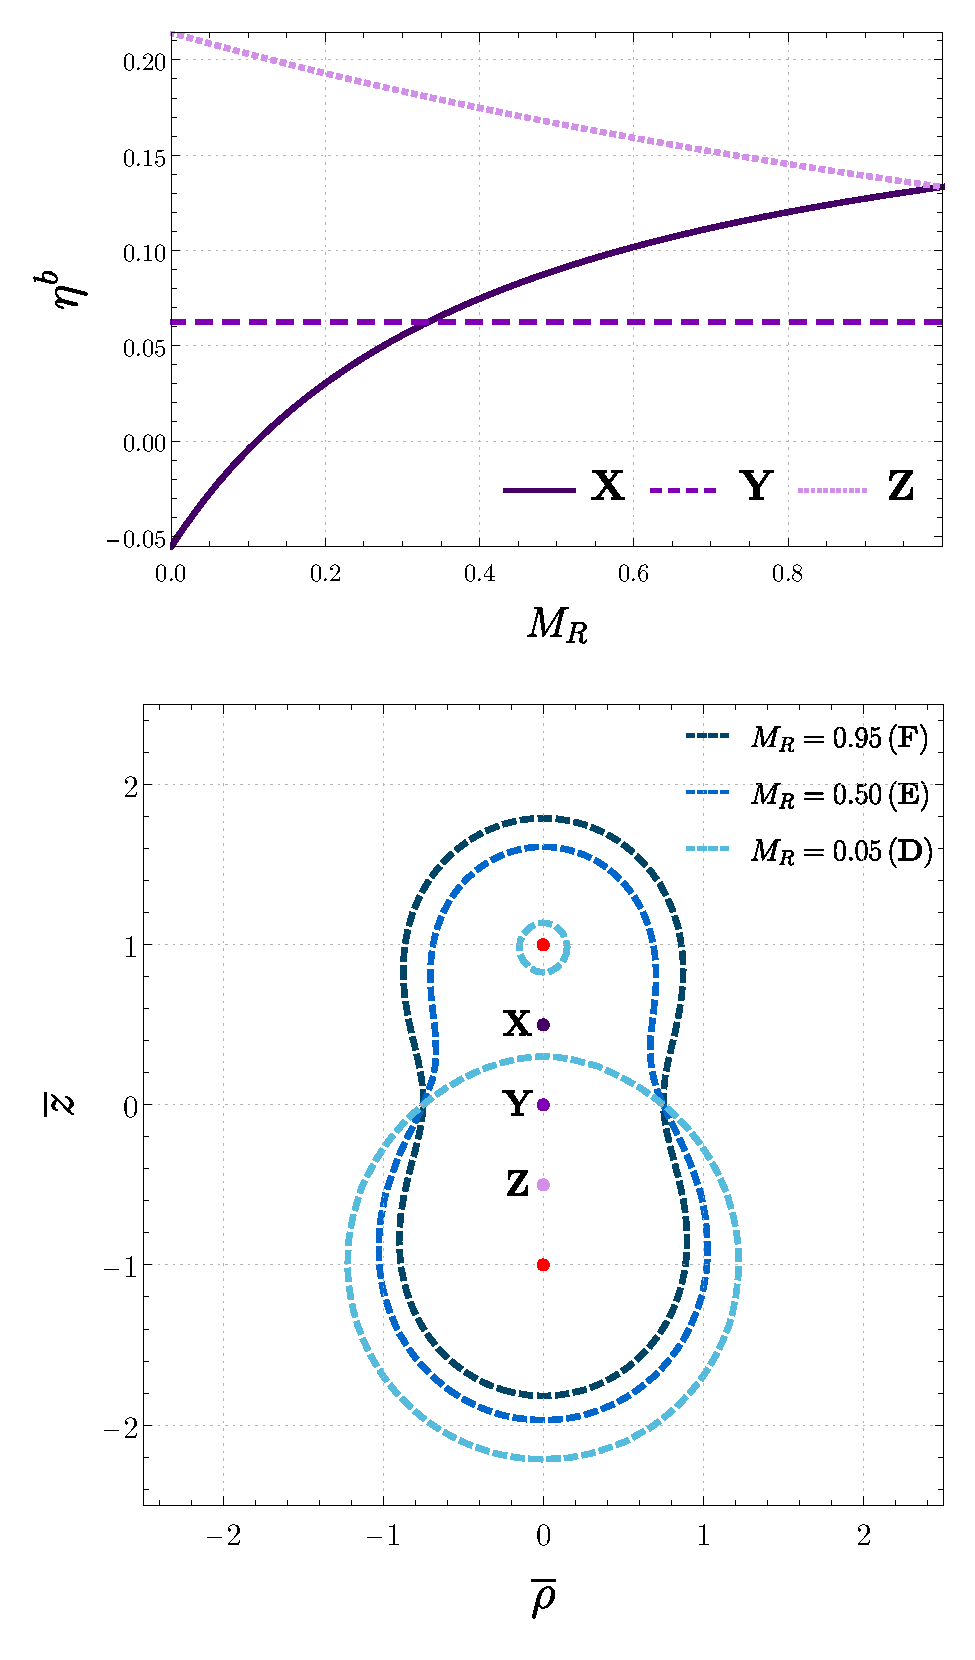
\includegraphics[scale=0.50]{img/penrose_binaries/fig8.pdf}
  \caption{Top panel: efficiency bound $\eta^{b}$ as a function of $M_R$ when $M_T/a=3$ and $\mu_{(1)} = -5/12$. Bottom panel: generalized ergosphere for selected values of $M_R$ (corresponding to the points  \textbf{D}, \textbf{E} and \textbf{F} in Fig.~\ref{fig:regions}) when $M_T/a=3$ and $\mu_{(1)} = -5/12$. The red dots indicate the location of the black holes. The purple dots are the locations of the break-up points $(\overline \rho_*,\overline z_*)=(1/2,1/2)$, $(\overline \rho_*,\overline z_*)=(1/2,0)$, and $(\overline \rho_*,\overline z_*)=(1/2,-1/2)$ and are labeled \textbf{X}, \textbf{Y} and \textbf{Z}, respectively. Each curve in the top panel corresponds to one of the break-up points shown in the bottom panel.}
  \label{fig:efficiency2}
\end{figure}

Finally, we investigate the behavior of $\eta ^{b}$ when $\mu_{(1)}$ and $M_T/a$ vary simultaneously, but their product, i.e. $\overline \mu_{(1)} = \mu_{(1)} M_T/a$, is kept fixed, meaning that the shape of the ergosphere is fixed (only the energy levels inside it change). In Fig.~\ref{fig:efficiency1} we plot $\eta^b$ as a function of $\mu_{(1)}$ and $M_T/a$ for three different break-up points when $M_R=1/2$ and $\overline \mu_{(1)} = -5/4$, so that the resulting ergosphere corresponds to the one labeled \textbf{E} in Figs.~\ref{fig:regions} and \ref{fig:ergos}. The break-up points are chosen to be $(\overline \rho_*,\overline z_*)=(d,1-d)$, with $d=1/2$, $d=1/3$, and $d=1/4$. We observe that, as $|\overline {\mu}|$ increases and $M_T/a$ decreases, the efficiency bound increases, approaching an asymptotic value in the limit $\mu_{(1)} \rightarrow -\infty$ and $M_T/a \rightarrow 0$.

\begin{figure}[h]
  \centering
  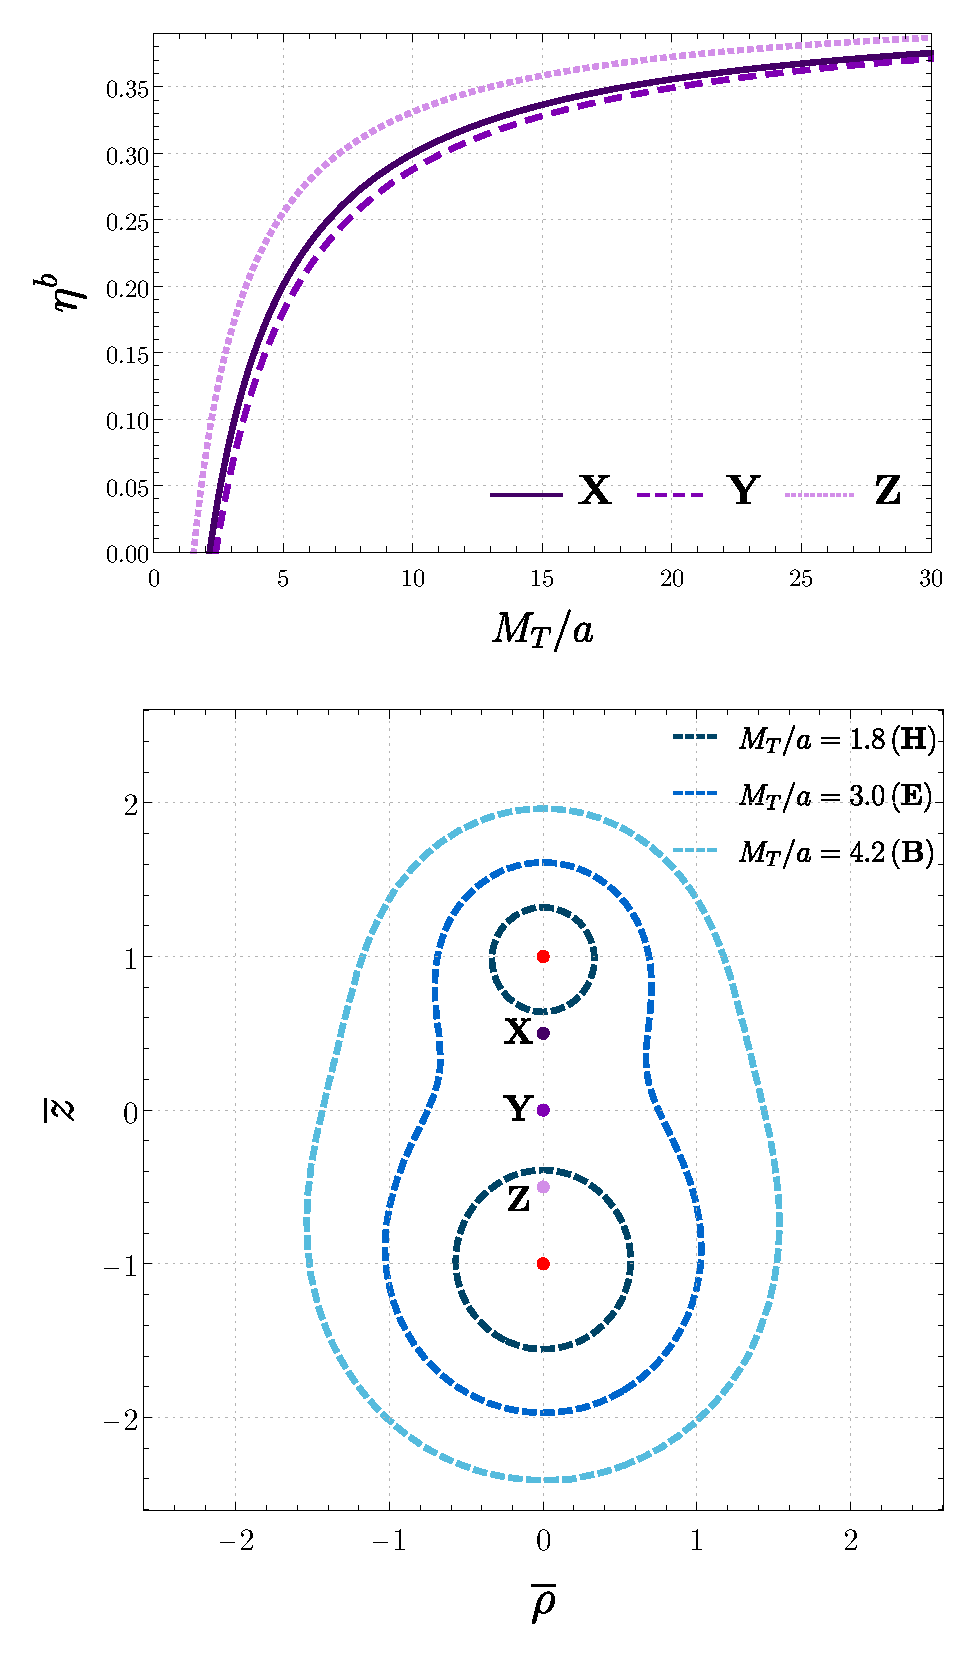
\includegraphics[scale=0.50]{img/penrose_binaries/fig9.pdf}
  \caption{Top panel: efficiency bound $\eta^{b}$ as a function of $M_T/a$ when $M_R=1/2$ and $\mu_{(1)} = -5/12$. Bottom panel: generalized ergosphere for selected values of $M_T/a$ (corresponding to the points  \textbf{B}, \textbf{E} and \textbf{H} in Fig.~\ref{fig:regions}) when $M_R=1/2$ and $\mu_{(1)} = -5/12$. The red dots indicate the location of the black holes. The purple dots are the locations of the break-up points $(\overline \rho_*,\overline z_*)=(1/2,1/2)$, $(\overline \rho_*,\overline z_*)=(1/2,0)$, and $(\overline \rho_*,\overline z_*)=(1/2,-1/2)$ and are labeled \textbf{X}, \textbf{Y} and \textbf{Z}, respectively. Each curve in the top panel corresponds to one of the break-up points shown in the bottom panel.}
  \label{fig:efficiency3}
\end{figure}

\begin{figure}[h]
  \centering
  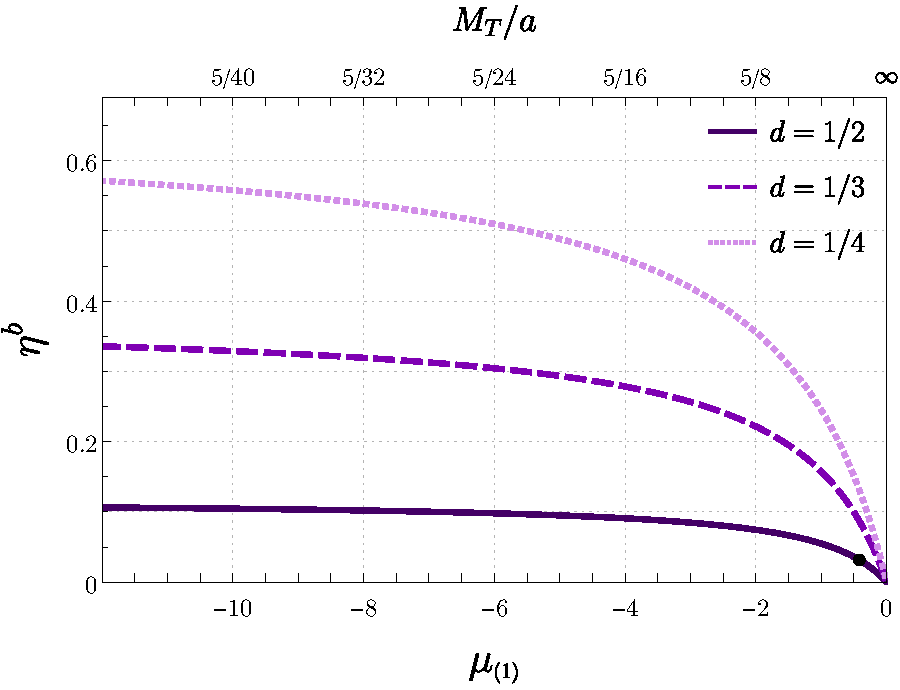
\includegraphics[scale=0.70]{img/penrose_binaries/fig10.pdf}
  \caption{Efficiency bound $\eta ^ b$ as a function of $\mu_{(1)}$ (bottom axis) and $M_T/a$ (top axis) for $M_R=1/2$ and $\overline \mu _{(1)} = -5/4$. The fact that $\overline \mu _{(1)}$ is fixed implies that $\mu_{(1)}$ and $M_T/a$ are inversely proportional to each other. The curves, from bottom to top, correspond to the break-up points $(\overline \rho_*, \overline z_*)=(d,1-d)$, with $d=1/2$, $d=1/3$, and $d=1/4$ respectively. The black dot shows the maximum efficiency $\eta^b = 0.03161$ for the processes represented in Fig.~\ref{fig:examplemax1} and Tables \ref{tab:max1} and \ref{tab:max2}, i.e.~when $d=1/2$, $\mu_{(1)} = - 5/12$ and $M_T/a=3$.}
  \label{fig:efficiency1}
\end{figure}

\subsection{Examples}

We now give concrete examples of energy extraction in a MP binary black hole spacetime whose efficiency approaches the theoretical maximum given by Eq.~\eqref{eq:eta_max_theory}. The general procedure that we follow is outlined below. First, we choose the MP parameters $M_1$, $M_2$ and $a$. Second, we choose the charge-to-mass ratio $\mu_{(1)}$ and a break-up point $(\rho_*,z_*,\phi_*)$ that is inside the generalized ergosphere of the spacetime. Without loss of generality, we set $m_{(0)}=1$.

Following the discussion leading to the inequality \eqref{eq:eta_max_theory}, we set $L_{(0)}=L_{(1)}=L_{(2)}=0$, meaning that all trajectories are restricted to the plane $\phi=\phi_*$. The energy $E_{(1)}$ is determined by Eq.~\eqref{eq:penrose_neg_energy}, while $E_{(0)}=1$. According to Eqs.~\eqref{eq:mu0max} and \eqref{eq:m1_max}, we choose
\begin{eqnarray}
  \label{eq:epsilondef} \mu_{(0)} &= 1 - \varepsilon, \\
  \label{eq:nudef} m_{(1)} &= 1 - \nu,
\end{eqnarray}
where $\varepsilon$ and $\nu$ are small positive parameters satisfying
\begin{equation} \label{eq:nuepsilonrelation}
  \nu > \varepsilon (U_* - 1) \left( \sqrt{1 + \frac{2}{\varepsilon (U_* - 1)}} - 1 \right).
\end{equation}
Since $m_{(1)}$  has been fixed, the mass $m_{(2)}$ can be determined by Eq.~\eqref{eq:mass2_eq2}. The quantities $\mu_{(2)}$ and $E_{(2)}$ are determined from Eqs.~\eqref{eq:charge_conservation} and \eqref{eq:conservation_of_energy}, respectively.

At the break-up point, according to Eq.~\eqref{eq:traj1}, we have $\dot \rho_{(1)}=\dot z_{(1)} = 0$ for the negative energy fragment. For the incident particle, on the other hand, the choices for $\mu_{(0)}$ and $E_{(0)}$ imply that
%
\begin{equation}\label{eq:velocity_eq_max_energy_example}
  \dot \rho_{(0)} ^2 + \dot z_{(0)} ^2 = \varepsilon \frac{U_*-1}{U_* ^2} \left[2 + \varepsilon (U_* - 1) \right].
\end{equation}
%
By choosing the angle $\theta_{(0)} = \mathrm{Arg}\left(\dot \rho_{(0)} + i \, \dot z_{(0)} \right)$ between the velocities $\dot \rho_{(0)}$ and $\dot z_{(0)}$, equation Eq.~\eqref{eq:velocity_eq_max_energy_example} can be used to determine $\dot \rho_{(0)}$ and $\dot z_{(0)}$ individually at the break-up point. The conservation of linear momentum then fixes the values of $\dot \rho_{(2)}$ and $\dot z_{(2)}$ through Eq.~\eqref{eq:conservation_mom_lin}. At this point, the trajectories $T_{(0)}$, $T_{(1)}$, and $T_{(2)}$ have all been determined and the efficiency of the associated Penrose process is $\eta=(1-\nu)\eta^{b}$.  In order to maximize the efficiency of the Penrose process, one must, therefore, set $\eta$ to be as small as possible. Note, however, that one cannot choose $\varepsilon=0$, because this would imply $\dot \rho_{(0)} = \dot z_{(0)} = 0$ and  $\ddot \rho_{(0)} = \ddot z_{(0)} = 0$ at the break-up point, contradicting the fact the trajectory $T_{(0)}$ starts infinitely far away. Similarly, $\nu$ cannot be chosen to saturate inequality \eqref{eq:nuepsilonrelation}, otherwise $m_{(2)}$ would be exactly zero, contradicting the fact that all trajectories are time-like. If desired, this can be remedied by assuming, from the start, that the escaping fragment is massless (however, this would modify Eq.~\eqref{eq:alternative_expression_for_energy} and the present analysis). Nevertheless, it is possible, in principle, to have infinitesimally small values for $\varepsilon$ and $\nu$. Finally, we point out that not every angle $\theta_0$ produces trajectories that are consistent with the assumptions of a Penrose process. More precisely, only certain ranges of $\theta_0$ give rise to trajectories  $T_{(0)}$ and $T_{(2)}$ that, respectively, start and end infinitely far away from the black holes.

\begin{figure}[h]
  \centering
  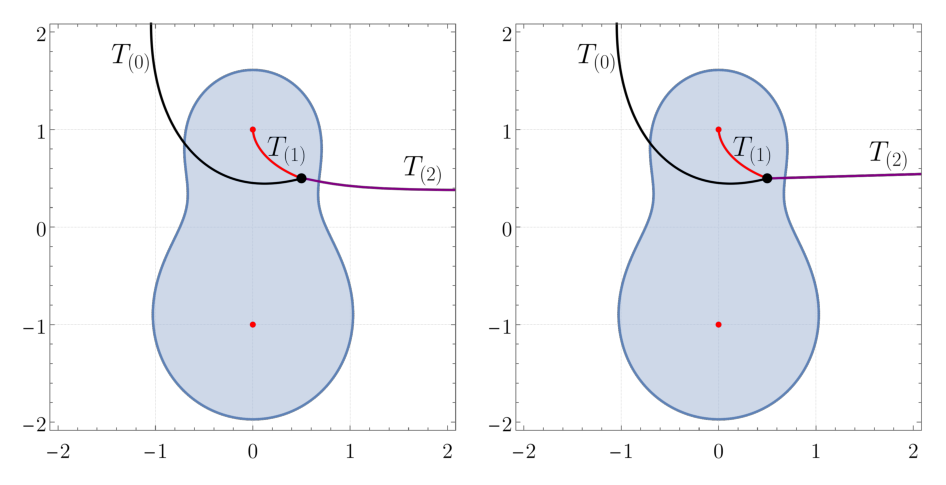
\includegraphics[scale=0.70]{img/penrose_binaries/fig11.pdf}
  \caption{Examples of Penrose processes that approach the maximum theoretical efficiency in a MP spacetime. The efficiencies of the processes in the left and right panel are, respectively, $90 \%$ and $99 \%$ of the theoretical maximum. In both cases the incoming trajectory $T_{(0)}$ (black curve) splits at the black point into the negative energy orbit $T_{(1)}$ (red curve) and the trajectory of the escaping fragment $T_{(2)}$ (purple curve). The parameters that generate these trajectories are shown in Tables \ref{tab:max1} and \ref{tab:max2}. The blue region is the generalized ergosphere (for particle 1) and the red dots indicate the location of the black holes.}
  \label{fig:examplemax1}
\end{figure}

\begin{table}[h]
  \centering
  \begin{tabular}{ccccccc}
    \hline\hline
    $i$ & $m_{(i)}$ & $\mu_{(i)}$ & $E_{(i)}$ & $L_{(i)}$ & $\dot{\rho}_{(i)}$ & $\dot{z}_{(i)}$ \\ \vspace{-0.3cm} \\
    0   & 1.00000   & 0.99990     & 1.00000   & 0         & 0.00609            & 0.00158         \\
    1   & 0.90000   & -0.41667    & -0.03161  & 0         & 0.00000            & 0.00000         \\
    2   & 0.09756   & 14.09301    & 10.54183  & 0         & 0.06243            & 0.01621         \\
    \hline\hline
  \end{tabular}
  \caption{Parameters that generate the trajectories $T_{(0)}$, $T_{(1)}$, and $T_{(2)}$ of the Penrose process shown in the left panel of Fig.~\ref{fig:examplemax1}. The derivatives $\dot{\rho}_{(i)}$ and $\dot{z}_{(i)}$ are evaluated at the break-up point.
  }
  \label{tab:max1}
\end{table}

\begin{table}[h]
  \centering
  \begin{tabular}{ccccccc}
    \hline\hline
    $i$ & $m_{(i)}$ & $\mu_{(i)}$ & $E_{(i)}$ & $L_{(i)}$ & $\dot{\rho}_{(i)}$ & $\dot{z}_{(i)}$ \\ \vspace{-0.3cm} \\
    0   & 1         & 0.99999     & 1.00000   & 0         & 0.00193            & 0.00050         \\
    1   & 0.99000   & -0.41667    & -0.03161  & 0         & 0.00000            & 0.00000         \\
    2   & 0.00685   & 206.13521   & 150.50460 & 0         & 0.28104            & 0.07297         \\
    \hline\hline
  \end{tabular}
  \caption{Parameters that generate the trajectories $T_{(0)}$, $T_{(1)}$, and $T_{(2)}$ of the Penrose process shown in the right panel of Fig.~\ref{fig:examplemax1}. The derivatives $\dot{\rho}_{(i)}$ and $\dot{z}_{(i)}$ are evaluated at the break-up point.
  }
  \label{tab:max2}
\end{table}

We conclude by showing in Fig.~\ref{fig:examplemax1} two explicit examples of the procedure outlined above for the MP spacetime with $M_1=2$, $M_2=1$, and $a=1$. The charge-to-mass ratio of the negative energy fragment is chosen as $\mu_{(1)}=-5/12$, so that the associated generalized ergosphere is the one identified by the letter \textbf{E} in Figs.~\ref{fig:regions} and \ref{fig:ergos}. The  break-up point is chosen as $(\rho_*,z_*)=(1/2,1/2)$, fixing the trajectory $T_{(1)}$ and its energy (per unit mass) $E_{(1)}=-0.03161$ (remember that the initial conditions are chosen so that $E_{(1)}$ is the minimum possible). According to Eq.~\eqref{eq:eta_max_theory}, the efficiency bound is $\eta^{b} = 0.03161$ (which corresponds to the black dots in Figs.~\ref{fig:efficiency0} and \ref{fig:efficiency1}). The trajectories $T_{(0)}$ and $T_{(2)}$ are specified by the choices of $\varepsilon$, $\nu$, and $\theta_{(0)}$. In the left panel of Fig.~\ref{fig:examplemax1}  we exhibit the Penrose process for $\varepsilon=10^{-4}$, $\nu=10^{-1}$, and $\theta_{(0)}=0.25403$, whose efficiency is $90 \%$ of the theoretical maximum. In the right panel of Fig.~\ref{fig:examplemax1} we exhibit the Penrose process for $\varepsilon=10^{-5}$, $\nu=10^{-2}$, and $\theta_{(0)}=0.25403$, whose efficiency is $99 \%$ of the theoretical maximum. The parameters that generate these examples and satisfy Eqs.~\eqref{eq:charge_conservation}-\eqref{eq:mass_constraint} are  given in Tables \ref{tab:max1} and \ref{tab:max2}.